\section{Goals and Methodology}
The IDDR implementation uses the \texttt{Linux kernel 3.5.0} for both application and driver domains. We tested it with Arch Linux on \texttt{x86\_64} platform. The specification of the system used for evaluation is presented in the table~\ref{tab:config}. 

\begin{center}
\begin{tabular}{|r|l|} 
  \hline
  \label{tab:config}
  System Parameter & Configuration \\
  \hline
  Processor & 2 X ??, ??.?? Ghz \\
  Number of cores & 4 per processor \\
  Hyperthreading & ?? \\
  Turbo boost & ?? \\
  L1 L2 cache & ??K/??K per core \\
  L3 cache & ?? X ??MB \\
  Main memory & ??GB \\
  Storage & SATA, HDD ??RPM \\
  \hline 
\end{tabular}
\end{center}
 
\subsection{Goals}
Our evaluation contains 
\begin{enumerate} 
\item comparison of Xen split driver and IDDR without any performance improvement, 
\item an evaluation of IDDR performance improvement over base IDDR system,
\end{enumerate}
The goal of this evaluation is to show that by avoiding the use of event channel in communication channel improves the performance of the system. 
\\
For performance measurement we use block devices such as ramdisk device, loop device, and SATA disk. We format the raw block device with ext2 file system, and in order to evaluate the performance of the Xen driver domain system, we run the fileIO SysBench benchmark~\cite{sysbench} on the mounted filesystem. Sysbench benchmark generates 128 files with ??GB of total data and performs random reads with a block size of 16KB. 

\section{Xen split driver vs IDDR}
We measure the performance of the xen split block device driver as the Xen driver domain follows the same architecture.
\subsection{Experimental setup}
\subsubsection*{Xen split driver}
We create a ramdisk in domain 0. The guest domain domU is configured to use the ramdisk as a disk. The guest domain domU uses the disk through split block device driver. We format and mount the the raw disk in guest domain with ext2 file system. Sysbench benchmark is run on the mounted disk.
\\[3mm]
We perform performance analysis with similar setup for loop device and SATA disk. For loop device, we create a loop device in domain 0 and then configure the guest domain to use loop device as a disk. For SATA disk, we configure the guest domain to use SATA disk as a secondary disk. 
\subsubsection*{IDDR}
In xen split block device driver setup, back end device driver runs in a domain 0 and front end device driver runs in a domain U. HVM guests are expected to have less syscall overhead and faster memory bandwith than PV guests. In our setup domain U is a HVM guest where as domain 0 is a PV guest. In order to have fair comparision it is necessary to run backend driver in a domain 0 and front end driver in domaun U.
\\[3mm]
We insert ramdisk and front end module in the domain 0 and insert the back end module in the guest domain domU. We format and mount the ramdisk with ext2 file system and sysbench benchmark is run on it.  
\\[3mm]
Similar setup is used for loop device and SATA disk.
\subsubsection*{Comparision}
\begin{figure}[!ht]
\centering
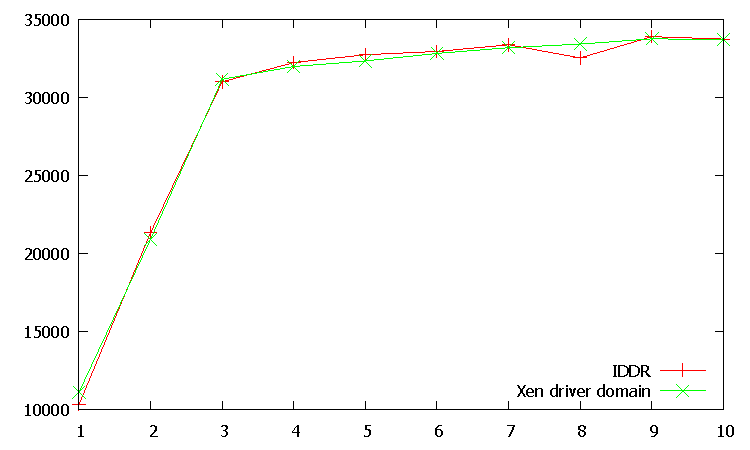
\includegraphics[scale=1]{iddrvsxen-ramdisk-rdwr}
\caption{IDDR vs Xen split driver}
\label{fig:iddrvsxen-ramdisk-rdwr}
\end{figure}
\begin{figure}[!ht]
\centering
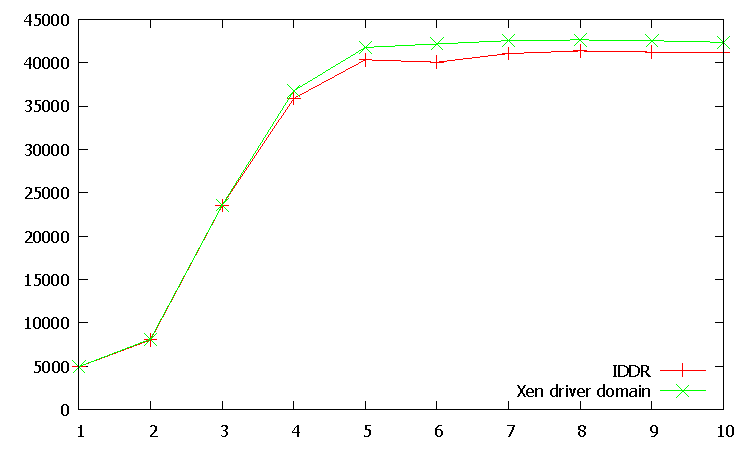
\includegraphics[scale=1]{iddrvsxen-loop-rd}
\caption{IDDR vs Xen split driver}
\label{fig:iddrvsxen-loop-rd}
\end{figure}
Figure~\ref{fig:iddrvsxen-ramdisk-rdwr} shows the performance for a random reads and random writes on ramdisk, and figure~\ref{fig:iddrvsxen-loop-rd} shows the performance for a random read on loop device. Both systems provide roughly similar performance. IDDR is the re-implementation of the Xen driver domain system, and performance of the IDDR is comparable to Xen driver domain. In further section we evaluate the performance improvement against IDDR system.

\section{IDDR performance improvement}
We measure and compare the performance of the IDDR system with context switch and the IDDR system without context switch. We run the fileIO sysbench benchmark with random reads, random writes, mixed random reads $\&$ random writes. 
\subsection{Experimental setup}
We create a ramdisk in a guest domain domU. We insert a back end driver in the guest domain and front end driver in the domain 0. In this setup, domain 0 is a Application domain, and domain U is a driver domain. We format and mount the the raw disk in application domain with ext2 file system. Sysbench benchmark is run on the mounted disk. 
Figure~?? shows the performance comparison of the IDDR system.
\\[3mm]
For loop device similar setup is created. We create a loop device in a driver domain, and insert back end driver in the driver domain. Front end driver is inserted in domain 0. For SATA disk, we passthrough SATA disk to driver domain, so that driver domain can directly access the SATA disk. 
\subsubsection*{Comparision}
\begin{figure}[!ht]
\centering
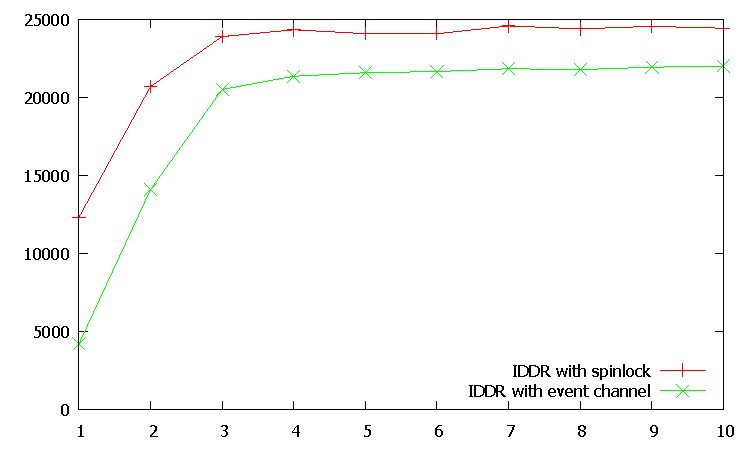
\includegraphics[scale=1]{threadvsspin}
\caption{IDDR with Spinlock vs IDDR with event channel}
\label{fig:threadvsspin}
\end{figure}
Figure~\ref{fig:threadvsspin} shows the performance for a random reads and random writes on ramdisk. Communication channel implementation with spinlocks performs better than base implementation with event channel. 

\pagebreak

% ref
\ifbool{toShowBibliography}{\bibliography{references}}{}